\documentclass[a4paper]{article}
\usepackage[left=3cm, right=3cm]{geometry}
\usepackage{hyperref}
\usepackage{cite}
\usepackage{amssymb}
\usepackage{url}
\usepackage{float}
\usepackage{longtable}
\usepackage{array}
\usepackage{algorithmic}
\usepackage[boxed]{algorithm}
\usepackage{color}
\usepackage{graphicx}
\pagestyle{headings}
\newcommand{\secondo}{\textsc{Secondo}}
\newcommand{\bmodb} {BerlinMOD Benchmark}
\newcommand{\op}[1]{\textbf{#1}}
\newcommand{\var}[1]{\textsl{#1}}
\newcommand{\dt}[1]{\textsl{\underline{#1}}}
\newcommand{\true}{\var{TRUE}}
\newcommand{\false}{\var{FALSE}}
%opening
\title{Network Data Model and BerlinMOD Benchmark}
\author{Simone Jandt}
\date{Last Update: \today}
\begin{document} 
\maketitle
\begin{abstract}
In the past several data models for the representation of spatial and spatio-temporal data objects have been developed. Among others we can categorise the data models into data models for objects moving freely in space and data models for moving objects that are constrained by a given network. For both categories several different data models have been developed. Two of them, one data model for objects moving freely in the 2D plane and one for network constrained moving objects have been implemented in \secondo{} DBMS. Both of them handling with the history data of moving objects. In this paper we present the comparison of the capabilities of the both data models using the \bmodb{}. The results show the advantages of specialised data models for network constrained objects. Therefore we propose a extension of the \bmodb{} with a additional query set BerlinMOD/Net including specialised challenges for network data models. This extensions enable us to compare the capabilities of different network data models with the \bmodb{}.
\end{abstract}
\section{Introduction}
In the past several data models for the representation of spatial and spatio-temporal data objects have been developed. Among others we can categorise them into data models for objects moving freely in space and data models for objects which movement is constrained by a network. For both categories several different data models have been presented like \cite{335426,chenzaniolosqlst} for spatio-temporal data objects moving freely in space and \cite{1146465,956692,VazWolfNetMod} for spatio-temporal data objects constrained by networks to name just a few.

For our experiments we choosed one example data model as representative for each of the both categories to compare the capabilities of the both different data models. The category of data models for spatio-temporal objects moving freely in space is represented by the data model presented in \cite{335426}. And the category of network data models is represented by the network data model presented in \cite{1146465}. The advantage of this choice is, that both data models are implemented in the \secondo{} DBMS and use the same temporal representation. So we can exclude that the use of different DBMS or temporal representations impact our results.

We used the recently introduced \bmodb{} \cite{BerlinMODVLDB} to compare the capabilities of the both data models. The \bmodb{} is best to our knowledge the first benchmark for complete spatio-temporal database systems and it is available in the \secondo{} DBMS. Furthermore the \bmodb{} data model is the data model of freely movement we use for our comparison. So we only have to transform the \bmodb{} spatial and spatio-temporal data types once in our network data model representation. This avoids sources of errors and relieves the control for correctness of the query results.

The results of our experiments show that it makes sense to use specialised network data models for network constrained objects, because the network data model outperforms the data model of free movement in the space in nearly all test cases. The total run time over all queries for the network data model is one-third of the total run time for the data model of free movement in the space. So the further developement of network data models seems to be useful. But network data models have their own challenges like network distance computing therefore we propose a extension of the \bmodb{} with a additional query set BerlinMOD/NET. This new query set should cover the specialised challenges of network data models. And enable us to compare the capabilities of different network data models also for the specialised network challenges with the \bmodb{}.

The rest of the paper is organised as follows. In section \ref{sec:relWork} we will first give short reminders of the underlying \secondo{} DBMS \ref{sec:secondo}, the \bmodb{} \ref{sec:bmodb} and the data models (\ref{sec:bmodbdatamod} and \ref{sec:netdatamod}) used in this paper. In section \ref{sec:bmodbNetDataMod} we present the setup for our experiments in \ref{sec:scenario} and describe our transfer of the \bmodb{} in the network data model representation in \ref{sec:Translation} before we show our experimental results in section \ref{sec:results}. In section \ref{sec:newqueries} we present our proposed extension of the \bmodb{} query sets. We conclude the paper with a summation of our results and aspects of future work in section \ref{sec:summary}.
\section{Related Work}
\label{sec:relWork}
As mentioned before in the past other data models for free movement in the space \cite{335426,chenzaniolosqlst} and for network constrained movement have been presented \cite{1146465,956692,VazWolfNetMod}. As well there are some more benchmarks \cite{COSTBenchmark, QueriesTheodoridis} and database systems for spatial and spatio-temporal datatypes \cite{HERMES,1054151}. But they don't provide a combination of different implemented and supported data types together with a existing benchmark like the actual \secondo{} DBMS. It is self-evident for us to use the \secondo{} DBMS in combination with the provided data types and benchmark to compare the capabilities of the both different representations of spatial and spatio-temporal data objects for network constrained objects.

In the next subsections we give short reminders of the used database system (\ref{sec:secondo}), the used benchmark (\ref{sec:bmodb}), and the used data models (\ref{sec:bmodbdatamod}, \ref{sec:netdatamod}). More detailed information for each of them can be taken from the original papers.
\subsection{Secondo}
\label{sec:secondo}
The extensible \secondo{} DBMS presented in \cite{686903,1054151} provides a platform for implementing various kinds of data models defining a clean interface between the data model independent system frame and the content of the single data models. The data model independent components and mechanisms are separated from the data model dependent parts. Hence \secondo{} can be easy extended by implementing \secondo{} algebra modules to provide new data types and operations by the user. The user also may define additional viewers for the graphical user interface or write optimisation rules or cost functions to extend the optimiser. \secondo{} is free available in the web \cite{secondoweb} and comes with a number of already implemented spatial and spatio-temporal data types and operations including the spatio-temporal data model of free movement in the space \ref{sec:bmodbdatamod} and the network data model \ref{sec:netdatamod} (since version 2.8.4). Furthermore the \bmodb{} descripted in \ref{sec:bmodb} has been developed in the \secondo{} DBMS. For our experiments we used the \secondo{} version 2.9.1 with some minor bugfixes in the NetworkAlgebra and the TemporalNetAlgebra.
\subsection{BerlinMOD Benchmark}
\label{sec:bmodb}
The \bmodb{} was recently presented in \cite{BerlinMODVLDB} \nocite{BerlinMOD} and is implemented in the \secondo{} DBMS. It is available in the web \cite{berlinmodweb} and provides a well defined data-set and queries for the experimental evaluation of different moving object data representations. The \bmodb{} emphasises the development of complete systems and simplifies experimental repeatability pointing out the weakness and the potency of the benchmarked systems.

The data-sets of the \bmodb{} are created using the street map of Berlin \cite{bbike} and statistical data about the regions of Berlin \cite{bevberlin,berlinstadtatlas} as input relations. The created moving objects represent cars driving in the streets of Berlin. This makes it possible to use the data set of the \bmodb{} also for network constrained data models. Every moving object has a home node and a work node and every weekday there will be a trip from the home node to the work node in the morning and trip from the work node back to the home node in the afternoon. In the evening and at the weekend randomly chosen cars spend additional trips (one in the evening and up to six at the weekend) to different randomly chosen targets. The number of observed cars and the duration of the observation period can be influenced by the user of the \bmodb{} by setting the \var{scalefactor} to different values in the data generation script. For example at \var{scalefactor} 1.0 the data generator will create 2000 moving objects observed for 28 days. Each of them sending a GPS-signal every 2 seconds. This simulated signals are simplified so that time intervals when a car doesn't move or moves in the same direction at the same speed are merged into one unit. E.g. if the car holds 8 hours in front of the work node there will be only one entry in the cars history of movement with a time interval of 8 hours instead of 14.400 entries one for each GPS interval.

The \bmodb{} provides two different approaches to store the histories of moving objects. On the one hand the object-based approach (OBA) and on the other hand the trip based approach (TBA). In the OBA the complete history for each object is kept together. In the TBA exist several trips for each object. In the OBA there is only one relation (dataScar) containing one tuple for each object consisting of the spatio-temporal data of the object (journey), the licence, the type, and the model of the object. In the TBA we have two relations. One of them (dataMcar) contains the static data for each object like licence, type, and model together with an object identifier. The other relation (dataMtrip) contains for each object identifier several tuples each of them containing a single trip of the moving object, whereby breaks between the trips (e.g. the time the car holds in front of the office) are stored as single (stationary) trips.

Besides the moving objects the \bmodb{} provides sets of \var{QueryPoints}, \var{QueryRegions}, \var{QueryInstants}, \var{QueryPeriods}, and \var{QueryLicences}, each of them containing 100 objects (points, regions, time instants, time intervals, and licences) used in the benchmark queries.

For this data objects the \bmodb{} provides two sets of queries. One set addresses range queries (BerlinMOD/R) and the  other one nearest neighbour queries(BerlinMOD/NN). In this paper we focus on the range queries which are the main aspect of the \bmodb{} up to now. The query set BerlinMOD/R includes 17 queries selected of the set of possible combinations of the 5 aspects object identity (known / unknown), dimension (standard / spatial / temporal / spatio-temporal), query interval (point / range / unbounded), condition type (single object / object relations), and aggregation (with or without aggregation). We will present the 17 queries in more detail in section \ref{sec:queries} together with our network data model translations.
\subsection{BerlinMOD Data Model}
\label{sec:bmodbdatamod}
The data model used by the \bmodb{} is the same data model of freely moving in 2D space presented in \cite{594784,335426,352963}. All spatial positions are given in x,y-coordinates. A single spatial position is represented by the data type \dt{point}. A \dt{point} consists of a pair of \dt{real} values interpreted as x,y-coordinates in the 2D plane. Streets are represented by \dt{line} values. A \dt{line} value consists of a set of half segments representing the geometry of the line in the 2D plane. Each half segment consists of two \dt{point} values which are interpreted as start and end point of the half segment. Regions are represented by the data type \dt{region}. A \dt{region} consists of a set of half segments interpreted as outer (and inner) border of the region in the 2D plane.

All this spatial data types and many standard data types can be lifted to become time dependent \dt{moving} values. For all data types \dt{$\alpha$} the constructor \dt{moving} creates a new data type \dt{moving}(\dt{$\alpha$}) (short form \dt{m$\alpha$}). A car may be represented by a \dt{mpoint}. A \dt{mpoint} is a \dt{point} changing its position within time. Therefore a \dt{mpoint} consist of a set of units called \dt{unit}(\dt{point}) (short form \dt{upoint}). Each \dt{upoint} consists of a time interval and two \dt{point} values. The first point represents the position of the \dt{mpoint} at the start of the time interval and the second point represents the position of the \dt{mpoint} at the end of the time interval. The \dt{point} is assumed to move on the straight line between this two points with constant speed. The speed is given by the ratio from the distance of the two points and the length of the time interval of the unit. All units of a \dt{mpoint} must have disjoint time intervals, because a car cannot be at two different positions at the same time. The units are sorted by ascending time intervals. This spatio-temporal data model of \dt{moving} allows us to compute the position of a \dt{mpoint} at every time instant within its definition time. We can also compute the time instant the point passed a given position assumed the \dt{mpoint} ever passes this position. The position of a \dt{point} at a given time instant is represented by a \dt{intime}(\dt{point}) (short form \dt{ipoint}). A \dt{ipoint} consists of a time instant and a \dt{point} value.

Some other data types of \secondo{} which are used in the \bmodb{} are shown in table \ref{tab:bmodbdatatypes}.
\begin{table}[H]
\begin{center}
\begin{scriptsize}
\begin{tabular}{|l|p{9.5cm}|}
\hline
\textbf{Data Type} & \textbf{Description} \\
\hline
\dt{bool} & Usual boolean data type.\\
\hline
\dt{int} & Usual integer number.\\
\hline
\dt{real} & Usual real number.\\
\hline
\dt{instant} & A point in time.\\
\hline
\dt{periods} & A set of disjoint and not connected time intervals.\\
\hline
\dt{mbool} & A time dependent boolean value. The value within each \dt{ubool} will be constant \true{} or \false{} \\
\hline
\dt{mreal} & Time dependent real number. Each unit will be defined by a function of time representing the \dt{real} value at each time instant.\\
\hline
\end{tabular}
\end{scriptsize}
\caption{Other Data Types of \bmodb{}}
\label{tab:bmodbdatatypes}
\end{center}
\end{table}
\subsection{Network Data Model}
\label{sec:netdatamod}
The central idea of the network data model presented in \cite{1146465} is that every movement is constrained by a network and every position is given related to this network. Therefore the data type \dt{network} is the central data type in the network data model. All other data types of the network data model are related to a \dt{network} by the unique network identifier that is part of each \dt{network} object. The \dt{network} object contains all spatial information of the represented network in three main relations. The first relation contains the attributes of the routes (streets) like id, route curve, route length, and two boolean flags indicating if the route starts at the lexicographic smaller end point and if the lanes of the route are separated like on German Highways or not. The second relation contains all attributes of the junctions (street crossings) like the identifiers of the first and second route crossing in the junction, the distance of the junction from the start of the first respectively second route, tuple identifiers of the both routes in the routes relation, tuple identifiers of the sections connected by this junction in the sections relation, and a connectivity code telling us which lanes of the two routes are connected by the junction. The third main relation of a \dt{network} object is the sections relation containing the attributes of the sections (street parts between two junctions or a junction and the end of the street) like the route identifier of the route the section belongs to, the tuple identifier of this route in the routes relation, start and end position of the section on the route, section curve, and two boolean flags \var{startssmaller} and \var{dual} with the same meaning as in the routes relation. We introduce four B-Tree indexes and one R-Tree index to support faster query execution. The four B-Trees indicate the route identifier attributes in the three main relations. And the R-Tree indicates the curve attribute of the routes relation. Furthermore there are two sets which provide a fast access from one section to their adjacent sections in driving direction\footnote{We call two sections adjacent if their lanes are connected by a junction.}.

Single positions in the network are given as \dt{gpoint} values. Besides the network identifier a \dt{gpoint} consists of a route identifier, a distance from the start of the route to the position of the \dt{gpoint} and a \dt{side} value ({\var{up}, \var{down}, \var{none}). The \dt{side} value is basically necessary if the route is dual, it tells us if the position is reachable form the \var{up} or the \var{down} \dt{side} of the route. For simple routes or positions which are reachable form both sides of the route the \dt{side} value is always \var{none}.

Parts of the network, regardless if they represent paths or regions, are given as \dt{gline} values. Besides the network identifier a \dt{gline} consists of a set of \dt{route intervals}, and two boolean flags telling us if the \dt{gline} is defined and if the set of \dt{route intervals} is sorted. Each \dt{route interval} consists of a route identifier identifying the route the \dt{route interval} belongs to, and the start and the end position from the \dt{route interval} on this route. In the original paper the \dt{route interval} includes a additional parameter \dt{side} like the \dt{gpoint} does. But this parameter is not part of the implementation yet. We call the \label{sec:sortedgline} set of \dt{route intervals} sorted if the following conditions are fullfilled:
\begin{enumerate}
	\item all \dt{route intervals} are disjoint
	\item the \dt{route intervals} are stored in ascending order of their route identifiers
	\item if two disjoint \dt{route intervals} have the same route identifier the \dt{route interval} with the smaller start position is stored first
	\item for all \var{route intervals} in the set the condition: $\var{start position} \le \var{end position}$ holds
\end{enumerate}
We introduced the sorted \dt{gline} because many algorithms take profit from sorted \dt{gline} values. For example the computation if a \dt{gpoint} is inside the \dt{gline} takes O(\var{n}) for unsorted and O($\log$ \var{n}) time for sorted \dt{gline} values, if \var{n} is the number of \dt{route intervals} in the \dt{gline}.

Unfortunately not all \dt{gline} values can be stored sorted. If a \dt{gline} value represents a path between two \dt{gpoint} in the network we need the \dt{route intervals} exactly in the sequence they are used in the path. This will nearly never be a sorted set like defined before. We solved this dilemma by introducing the sorted flag. Every algorithm which can take profit from a sorted \dt{gline} values checks this flag and uses the corresponding code. We store  \dt{gline} values sorted whenever this is possible to support faster query execution.

Mostly similar to the \dt{mpoint} of the other data model we implemented a \dt{mgpoint}. A \dt{mgpoint} consists of a set of \dt{ugpoint} with disjoint time intervals. Each \dt{ugpoint} consists of a time interval and two \dt{gpoint} values. Every time the \dt{mgpoint} changes the route or the speed a new \dt{ugpoint} is written. Each \dt{ugpoint} is assumed to follow the same route from the start to the end position at the same speed. So accordingly to the \dt{mpoint} we can compute the network position of the \dt{mgpoint} at ever time instant within the definition time of the \dt{mgpoint} as \dt{intime}(\dt{gpoint}).

In deviation from the original network data model we extended the implementation of the \dt{mgpoint} with four additional attributes:
\begin{enumerate}
	\item The total driven distance
	\item A sorted set of \dt{route intervals} representing the positions ever traversed by the \dt{mgpoint}
	\item A boolean defined flag for the set of \dt{route intervals}
	\item A spatio-temporal minimum bounding box
\end{enumerate}
The sorted set of \dt{route intervals} was introduced, because it makes it much faster to decide if a \dt{mgpoint} ever passed a given place or not. Instead of a linear check of all \var{m} \dt{ugpoint}s of a \dt{mgpoint} we perform a binary scan on the much lower number \var{r} of \dt{route intervals}. This reduces the time complexity from O(\var{m}) to O($\log \var{r}$) for all \op{passes} operations. Logical this should be done by a sorted \dt{gline} value but the \secondo{} DBMS restricts us to use a sorted set of \dt{route intervals} instead.

The spatio-temporal minimum bounding box was introduced as parameter to the \dt{mgpoint} because the computation of this value is very expensive in the network data model. Although each unit of a \dt{mgpoint} stays on the same route at same speed the motion may follow different spatial directions, e.g. a route may lead uphill in serpentine. Not all this positions must be enclosed by a bounding box computed just from the spatial position of the \var{start} and \var{end} position of the unit. Therefore we have always to examine the spatial dimensions of the complete part of the route passed within a unit to compute the units bounding box. All spatial information of the route curve is hidden in the \dt{network} object. We have to call the route curve from the \dt{network} object to compute the spatial dimensions of the unit bounding box. If \var{r} is the number of routes of the network and \var{h} the number of half segments of the traversed part of the route curve passed in a unit we need O($\log \var{r} + \var{h}$) time to compute the bounding box for a single unit. The bounding box of the \dt{mgpoint} is the union of the bounding boxes of its \var{m} units. So the computation of a \dt{mgpoint} bounding box takes O($\var{m}(\var{h} + \log r)$) time. This is very expensive therefore the bounding box of a \dt{mgpoint} is only computed on demand or if we can get it for free. E.g. we can copy the bounding box of a \dt{mpoint} if we translate it into a \dt{mgpoint} without computational effort. But we don't maintain this attribute at every change of the \dt{mgpoint}. If the \dt{mgpoint} changes we set the bounding box attribute to be undefined and compute it again on demand if necessary.
\section{BerlinMOD and Network Data Model}
\label{sec:bmodbNetDataMod}
In the next subsections we first present our experimental setup (\ref{sec:scenario}) and the transfer from the \bmodb{} data-sets and queries in our network data model representation including a description of the indexes we build to support faster query execution (\ref{sec:Translation}) before we conclude the section with the results of our experiments in \ref{sec:results}.
\subsection{Experimental Setup}
\label{sec:scenario}
For our experiments we used a Standard PC with a Intel Pentium 4 2.93 GHz CPU, 1 GB main memory, 200 GB HDD, and Linux openSUSE 11.1 as operating system. We installed \secondo{} version 2.9.1+ and the \bmodb{} from the web.

We used the data generating script of the \bmodb{} with \var{scalefactor} value 0.05, 0.2, and 1.0 to generate three data sets with different amounts of data in three different database directories. After that we build the index structures used by the \bmodb{} with the script ``BerlinMOD\_CreateObjects.SEC'' delivered with the \bmodb{} data for each database and started the benchmark queries for the object oriented and the trip based approach of the \bmodb{} on this databases. We saved the results for each database and measured the run times of the queries several times to be sure that the run times measured are free from other influences.

Next we translated the three databases into network data model representation. Therefore we build a \dt{network} object from the data of \var{streets relation} and  translated all spatial and spatio-temporal data types of the \bmodb{} data sets relative to this \var{network} object. We also defined some indexes to support faster query execution on the network data model representation and formulated executable \secondo{} queries for each BerlinMOD/R query on this network data set. We give a detailed description of the translation steps, indexes and queries in section \ref{sec:Translation}.
\begin{figure}
\begin{center}
	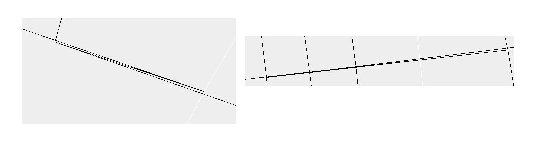
\includegraphics[scale=1.0]{routefailure.eps}
	\caption{Example Failures in Street Map}
	\label{fig:routefailure}
	\end{center}
\end{figure}
After that we started a first run of our network queries and compared the results of our network queries with the results of the \bmodb{} queries to ensure that all results are correct. We found some isolated missmatches in some query results, which are caused by the fact that singular route curves in the source data of the street map was not well defined see figure \ref{fig:routefailure} at two places. We corrected the source file ``streets.data`` delivered by \bmodb{} at this two routes and restarted the building of the databases and our experiments from the start. After all results from the network queries corresponded to the results of the \bmodb{} results we started the network queries several times to measure the run times analogues to the run times of the benchmark queries. The results of the run time measurement are shown in \ref{sec:results}.
\subsection{Translation of BerlinMOD into Network Data Model}
\label{sec:Translation}
In section \ref{sec:createNetwork} we describe the construction of the central \dt{network} object from the \var{streets} value of the \bmodb{}. This \dt{network} object is necessary to transfer the spatial and spatio-temporal data objects into the network data model representation like described in section \ref{sec:translateSTdata}. In section \ref{sec:createIndex} we describe the indexes we build on the data sets in the network data model to support a faster execution of the queries described in section \ref{sec:queries}.

A \secondo{} script for the network data creation and the translation of the \bmodb{} data sets into network data representation and \secondo{} scripts with the executable \secondo{} \bmodb{} queries on the network data model translation can be taken from our website \cite{berlinmodweb}.
\subsubsection{Create Network Object}
\label{sec:createNetwork}
We extract the routes data from the \var{streets} of the \bmodb{} data set to create a \dt{network} object for our network data model representation of the \bmodb{}. The extracted routes data \var{r} is used to compute the crossings of the routes of Berlin \var{j}. In this step the connectivity code for each crossing is set to the maximum value because the data source lacks on information about the connectivity of the crossings. We use \var{r} and \var{j} as input relations for the creation of our \dt{network} object \var{net} representing the streets of Berlin in the network data model.

The network creation algorithm first copies all tuples of \var{r} to the \var{routes relation} of \var{net} and creates the B-Tree index of the route identifiers and the R-Tree of the route curves of the \var{routes relation} of \var{net}. Then it copies all tuples of \var{j} to the \var{junctions relation} of \var{net} and adds the \var{tuple identifiers} for the both routes connected by this junction to the junctions entry in the \var{junctions relation}. After that two B-Trees indexes for the route identifiers of the first respectively second route in the \var{junctions relation} are build. Next for every route of the \var{routes relation} all junctions \var{jr} on this route are taken to compute for each of this junctions the up and down sections on the route. The up and down sections are inserted into the \var{sections relation} of \var{net} and the \var{tuple identifiers} of the sections are added to the entry of the according junctions in the \var{junctions relation}. After that the B-Tree index for the route identifiers in the \var{sections relation} is created and the  adjacency lists of \var{net} are filled with the adjacent section pairs defined by the \var{junctions relation}.

If $|\var{r}|$ is the number of routes and $|\var{j}|$ is the number of junctions. The algorithm needs O($|\var{r}| \log |\var{r}|$) time to copy \var{r} to the \var{routes relation} of \var{net} and create the trees indexing the \var{routes relation} of the \var{net}. The creation of the \var{junctions relation} and the build of the B-Trees indicating the route identifiers in this relation takes O($|\var{j}| \log |\var{j}|$) time. O($|\var{r}||\var{j}|$) time is needed to fill the \var{sections relation} and O($|\var{j}|$) time to fill the \var{adjacency lists} of \var{net}. Alltogether the complete algorithm needs: O($|\var{r}| \log |\var{r}|+|\var{j}| \log |\var{j}| + |\var{r}||\var{j}|$) = O($|\var{r}||\var{j}|$) time to create the \var{net} from the two input relations \var{r} and \var{j}.
\subsubsection{Translate Spatial and Spatio-Temporal Data}
\label{sec:translateSTdata}
We translate the spatial and spatio-temporal data types of the \bmodb{} data set into network objects related to the \dt{network} object \var{net} described in \ref{sec:createNetwork}. The input for all algorithms is a spatial respectively spatio-temporal object and the \dt{network} object to which they should be related. If a input data object is not constrained by the given \dt{network} object the result of the translation is undefined for all translation algorithms described in the following paragraphs.

We start explanation of our translation algorithms with the \op{point2gpoint} operation, because this operation is used by the other translation algorithms. The algorithm translates a \dt{point} value \var{p} into a corresponding \dt{gpoint} value by using the R-Tree index of the \var{network routes relation} to select the route closest to \var{p} and computes the position of \var{p} on this route. The \dt{side} value of the resulting \dt{gpoint} is always set to \var{none}. If \var{r} is the number of routes in the \var{network routes relation} and \var{k} is the number of possible candidate routes the worst case complexity of the algorithm is O($\var{k} + \log \var{r}$).

This should be all to translate the \dt{point} values of the \var{QueryPoints} relation of the \bmodb{} into network query positions. But we have a problem with the network data model representation of junctions. In the network data model contrary to the data model of freely moving in space junctions have more than one \dt{gpoint} representation, because they are related to two or more routes. Hence if a junction position is given related to route \var{a} we won't detect the junction as passed if a \dt{mgpoint} object passes the junction on route \var{b} in all cases, because the definition of \op{passes} in the network data model is slightly different from the \op{passes} operation in the \bmodb{} data model. Unfortunately all query points of the \bmodb{} are junctions. As work around we added a operator \op{polygpoints}, which returns for every input \dt{gpoint} value \var{gp} a stream of \dt{gpoint} values. If \var{gp} represents a junction we return all \dt{gpoint} values representing the same junction in the \dt{network} object, otherwise we return only \var{gp} in the stream. So we got 221 query \dt{gpoint} values in \var{QueryPointsNet} for the 100 query \dt{point} values in \var{QueryPoints} and 22 \dt{gpoint} values in \var{QueryPoints1Net} for the 10 \dt{point} values of \var{QueryPoints1} of the \bmodb{}. Although we have always to compute the results for the doubled number of query points our network data model outperforms the data model of free movement in nearly all cases by orders of magnitudes.

The second operation \op{mpoint2mgpoint} translates a \dt{mpoint} value \var{s} into a \dt{mgpoint} value \var{t}. The main idea of the algorithm is to use the continuous movement of \var{s} to reduce computation time. We initialise the algorithm by reading the first unit of \var{s} and use the \op{point2gpoint} operation to find a route in the network containing the \var{start point} and the \var{end point} of this unit. We initialise the first unit of \var{t} with the computed network values. Then we read each unit of \var{s} and try to find the \var{end point} of the unit on the same route the last unit of \var{s} was found. If the \var{end point} is found on this route we check the direction and speed of the unit. If they are equal to the last unit we extend the actual unit of \var{t} to enclose the value of the actual unit of \var{s}. If the speed or the moving direction changes we write the actual unit to \var{t} and initialise a new unit for \var{t} with the network values of the actual unit from \var{s}. If the \var{end point} cannot be found on the same route than the last unit from \var{s} we write the actual unit of \var{t} and start a search on the route curves of the adjacent sections to find the route curve that contains the \var{start point} and the \var{end point} of the actual unit of \var{s}. We initialise a new unit for \var{t} with the estimated network values for the actual unit of \var{s} and continue with the next unit of \var{s}. At least we add the actual network unit to \var{t}. The time complexity to find the start values for the first unit is O(\op{point2gpoint}). For the next \var{m} units of the \var{mpoint} the worst case complexity is O(\var{a}) for each unit if \var{a} is the maximum number of adjacent sections. So we get a worst case time complexity of O(O(\op{point2gpoint}) + \var{ma}) for the translation of a \dt{mpoint} into a \dt{mgpoint}.

The translation of the \dt{region} values in the \var{QueryRegions} relation of the \bmodb{} into \dt{gline} values of our network data model is done in several steps. First of all we build a single big \dt{line} object from all our network streets. Then we compute for each \dt{region} of the \var{QueryRegions} the intersection with this big \dt{line} object. At least we translate the resulting \dt{line} objects of the intersection, each representing one \dt{region} of the \var{QueryRegions} relation, into sorted \dt{gline} values using the \op{line2gline} operation. The algorithm of the \op{line2gline} operation takes each \dt{half segment} of a \dt{line} value and computes a corresponding network \dt{route interval} by searching a common route curve for the \var{start point} and the \var{end point} of the \dt{half segment} using the \op{point2gpoint} operation. The computed \dt{route intervals} are sorted, merged and compressed before the resulting \dt{gline} value is returned. If the number of \dt{half segments} of a \dt{line} value is \var{h} and the number of resulting compressed \var{route intervals} is \var{r} we get a time complexity of  O($\var{h}$O(\op{point2gpoint})$+ \var{h} \log \var{r} + \var{r}$) for the whole algorithm. Whereby the summand $\var{h} \log \var{r} + \var{r}$ is caused by the compressing and sorting of the resulting \dt{gline} but as mentioned before in \ref{sec:sortedgline} we think this time is well invested.
\subsubsection{Create Indexes on Network Data Model}
\label{sec:createIndex}
After translating all the \bmodb{} data sources we are able to create indexes on our network data representation of the \bmodb{} data. First we create B-Trees for the \var{licences} and \var{moid} attributes of the relations \var{dataSNcar}, and \var{dataMNtrip} similar to the indexes created in the \bmodb{} for \var{dataSCcar}, and \var{dataMCtrip}, because the relations \var{dataSNcar} and \var{dataMNtrip} contain the network data model representation of the \var{dataScar} and \var{dataMtrip} relation of the \bmodb{}. Then we create R-Tree indexes over the spatio-temporal bounding boxes of the \dt{mgpoint} attributes in the \var{dataMNtrip} and the \var{dataSNcar} relation. At least we create some specialised network indexes indicating network positions and network-temporal positions of moving objects. Therefore we introduced two and three dimensional \dt{netboxes}. A \dt{netbox} is a degenerated two or three dimensional rectangle. The coordinates of the rectangle are defined to be $x_1 = x_2 = $ \var{route identifier} as \dt{real} value (The equality of $x_1$ and $x_2$ makes the degeneration.), $y_1 = $ min(\var{start position}, \var{end position}), $y_2 = $max(\var{start position}, \var{end position}), and, in the three dimensional case, $z_1 =$  \var{start time} as \dt{real} value and $z_2 = $ \var{end time} as \dt{real} value.  For every unit of each \dt{mgpoint} we build a three dimensional \dt{netbox} and for every \var{route interval} of every \dt{mgpoint} a two dimensional \dt{netbox}. This \dt{netboxes} are used to create R-Trees over the network and network-temporal positions of the \dt{mgpoint}s in the network data representation of the \bmodb{}.
\subsubsection{Translate Benchmark Queries}
\label{sec:queries}
We developed executable \secondo{} queries for each of the 17 BerlinMOD/R queries for the object and the trip based approach using our network indexes to support faster query execution. We had to do this manually because the \secondo{} optimiser is not able to optimise SQL-queries on network data model objects yet. In our experiments we tried many different query formulations for each query to get optimal queries delivering the correct result in a minimum of time. The limited space does not allow us to show all our executable \secondo{} network queries in detail. As mentioned before the complete \secondo{} scripts can be taken from our website. In the following we describe only the algorithms of a view queries in detail.

Every time we need a licence in the result or have a query licence number we have a additional step in the TBA. Because we have to join the \var{trip} attribute from \var{dataMNtrip} with the \var{licence} attribute from \var{dataMNcar} using the \var{moid} attribute and the corresponding B-Tree indexes. This will not be repeated at every single query description.

Query 1 and 2 work only on standard attributes. They are formulated analogous to the original queries of the \bmodb{} only the relation names and the btrees are changed to match the network data model.

Query 3 selects uses the licence B-Tree to select the ten cars with licences from \var{QueryLicences1} from \var{dataSNcar} then the positions of this cars are computed for each of the ten time instants from \var{QueryInstants1}.

In Query 4 we produce a \var{netbox} for each of the \var{QueryPointsNet} and use our specialised netbox R-Tree of the \dt{route intervals} of the \dt{mgpoint} to select the passing vehicles.

In the queries 5, 6, and 10 a retransmission of network objects into spatial respectively spatio-temporal objects of the \bmodb{} data model is done. This is caused by the fact that the \bmodb{} deals with Euclidean Distances. Euclidean Distances are not very useful in network environments because all objects are restricted to use network paths. Therefore in networks normally the Network Distance is computed. To make the results comparable we retransmit the intermediate results of our network data model into spatial and spatio-temporal data types an use the existing spatial and spatio-temporal Euclidean Distance Functions of the \bmodb{} data model for the distance computation in the queries 5, 6, and 10. 

Query 5 selects the cars with \var{licences} from \var{QueryLicence1} respectively \var{QueryLicences2} using the B-Tree over the \texttt{Licence} attribute of \var{dataSNcar} and creates a \dt{line} value from the list of \dt{route intervals} passed by every car. Then the Euclidean Distance between this \dt{line} values is computed for each pair of licences one from \var{QueryLicences1} and one from \var{QueryLicences2}. In the TBA we need a aggregation step building the union of the several \dt{mgpoint} belonging to each candidate car. This is done with the \var{route intervals} because it takes much less time to build the union of the \dt{route intervals} than of the \dt{half segments} in the \dt{line} values representing the same network part.

Query 6 uses the \op{filter} operation to select the ''trucks`` from \var{dataSNcar} (respectively \var{dataMcar} in TBA) relation. Then the spatio-temporal bounding box of each trip is computed and the spatial dimensions of this box are extended by 5m in every spatial direction. After that the \dt{mgpoint} values are retranslated into \dt{mpoint} values. In a second step each result of the first step is joined with all other results of the first step if the extended bounding boxes intersect, the licences are different and the \dt{mpoint} values have sometimes a distance lower than 10m. The licence pairs of trucks fullfilling this predicate are returned. In the TBA there might be duplicate licence pairs which we have to remove before we return the result.

The first part of the first step of query 7 is almost equal to the selection of cars passing a query point in query 4. The intermediate result is filtered to remove all ``not passenger'' cars and for every remaining trip the time the trip reaches first the query position is computed for every query position and every candidate trip. In a second step the resulting time instants are grouped by the \var{id} of the query positions and the minimum time stamp of each group is computed. This minimum time stamp is for every query position the first time it was reached by a car. In the third and last step the licences of the cars reaching the query positions at this first time instant are computed by a join of the results of the first two steps by query position id and the equality of the time stamps.

In query 8 we just select the candidate cars with the licence B-Tree and compute for every car the length of the trip at the query periods in the OBA. In the TBA we have to aggregate over all the distances driven in the single trips by a car within a query period.

For query 9 we compute the length of every trip in every query period, and select the maximum driven distance for every period. In the TBA again we have to do a aggregation of the distances driven from the same car in the same period.

For query 10 we first retranslate every \dt{mgpoint} value of \var{dataSNCar} into a \dt{mpoint} value. In the OBA we extend the spatial bounding box of each of this both trips by 1.5 m in every direction. Second we select the ten candidate trips given by \var{QueryLicences1}, retranslate them and extend their spatial bounding boxes. Than we use \op{symmjoin} to join all trips from the first and the second step where the extended bounding boxes intersect. We filter the pairs that have different licences and are sometimes nearer than 3 m. For this pairs we compute the position of the \dt{mgpoint} at the times the distance between the both \dt{mpoint} has been smaller than 3 m. We return the licence pairs and the positions when they have been closer than 3 m to each other. Again we have to do in the TBA a aggregation of the resulting trips for each licence pair into one. We tried out several indexes to support faster query execution of query 10 including the MON-Tree \cite{MONTree}. But at least this simple form shows the best performance of all.

In query 11 we build a network-temporal query box from the product of \var{QueryInstant} and \var{QueryPoints1Net} relation. And use the network-temporal index on \var{dataSNcar} (respectively \var{dataMNtrip}) to select the resulting trips.

The first step of query 12 is identical with query 11. In a second step a product of the result of the first step with itself is computed and checked for vehicles which have been at the same query point at the same query time instant.

Query 13 first computes a network-temporal box for the query values and then uses this computed boxes to select the candidates with help of the network-temporal R-Tree. In TBA again the resulting \var{moids} must be mapped to the licences of the cars to generate the result.

Query 14 and 15 work almost similar to query 13 only the query value building the netboxes are different.

Query 16 selects the candidate trips using the licence B-Tree and filters them by the \op{passes} operation and restricts them to the times they were inside the query region. Then this reduced trips are filtered to be \op{present} within the query periods and are restricted to the times of the query periods. This is done twice. One time for \var{QueryLicences1} and one time for \var{QueryLicences2}. The both results are joined to get the trips of different cars which where at the same period in the same region without meeting each other there in a third step. Again in the TBA we have to do a additional selection from trips with the \var{moids} belonging to the cars selected before by the licences and to remove duplicates of licence pairs in the same period.

Query 17 again uses the methods from query 4 to find the trips passing a given query point. The passing cars are grouped by the passed query points and the number of cars per query point is computed. In a second step the point with the maximum number of hits is selected and his id and the number of passing cars is returned. In the TBA we have to remove the duplicate cars from the result before computing the hits.
\subsection{Benchmark Results}
\label{sec:results}
We made several runs for each data amount and each query to get correct average execution times for each query in both data models. The tables \ref{tab:rtbmodb} and \ref{tab:rtnet} show the resulting run times for each query in seconds. Figure \ref{fig:compruntimesall} visualises the run time comparison between the different data models and approaches.
\begin{table}
\begin{scriptsize}
\begin{center}
\begin{tabular}{|c|r|r|r|r|r|r|}
\hline
&\multicolumn{2}{c|}{\textbf{Scalefactor 0.05}}&\multicolumn{2}{c|}{\textbf{Scalefactor 0.2}}&\multicolumn{2}{c|}{\textbf{Scalefactor 1.0}}\\
\hline
\textbf{Query}&\textbf{OBA}&\textbf{TBA}&\textbf{OBA}&\textbf{TBA}&\textbf{OBA}&\textbf{TBA}\\
\hline
\textbf{1}&0.173&0.213&0.160&0.152&x.xxx&x.xxx\\
\hline
\textbf{2}&0.006&0.006&0.011&0.007&x.xxx&x.xxx\\
\hline
\textbf{3}&0.751&0.531&1.491&0.557&x.xxx&x.xxx\\
\hline
\textbf{4}&22.365&39.873&158.999&214.883&x.xxx&x.xxx\\
\hline
\textbf{5}&2.351&3.937&5.892&7.607&x.xxx&x.xxx\\
\hline
\textbf{6}&49.187&36.910&246.216&320.830&x.xxx&x.xxx\\
\hline
\textbf{7}&34.860&37.560&514.199&239.386&x.xxx&x.xxx\\
\hline
\textbf{8}&0.893&0.955&2.768&2.583&x.xxx&x.xxx\\
\hline
\textbf{9}&245.831&610.944&741.497&3282.183&x.xxx&x.xxx\\
\hline
\textbf{10}&326.769&141.512&1604.588&1141.317&x.xxx&x.xxx\\
\hline
\textbf{11}&0.186&0.249&1.572&0.818&x.xxx&x.xxx\\
\hline
\textbf{12}&1.843&0.287&118.927&0.349&x.xxx&x.xxx\\
\hline
\textbf{13}&36.509&36.148&350.815&164.260&x.xxx&x.xxx\\
\hline
\textbf{14}&1.372&1.701&14.816&8.656&x.xxx&x.xxx\\
\hline
\textbf{15}&3.143&3.387&115.370&48.872&x.xxx&x.xxx\\
\hline
\textbf{16}&89.351&38.791&62.673&70.790&x.xxx&x.xxx\\
\hline
\textbf{17}&3.600&17.825&179.519&195.433&x.xxx&x.xxx\\
\hline
\textbf{Total}&819.190&970.737&4119.612&5698.686&x.xxx&x.xxx\\
\hline
\end{tabular}
\end{center}
\end{scriptsize}
\caption{Query Run Times \bmodb{}}
\label{tab:rtbmodb}
\end{table}
\begin{table}
\begin{scriptsize}
\begin{center}
\begin{tabular}{|c|r|r|r|r|r|r|}
\hline
&\multicolumn{2}{c|}{\textbf{Scalefactor 0.05}}&\multicolumn{2}{c|}{\textbf{Scalefactor 0.2}}&\multicolumn{2}{c|}{\textbf{Scalefactor 1.0}}\\
\hline
\textbf{Query}&\textbf{OBA}&\textbf{TBA}&\textbf{OBA}&\textbf{TBA}&\textbf{OBA}&\textbf{TBA}\\
\hline
\textbf{1}&0,128&0.161&0.361&0.179&x.xxx&x.xxx\\
\hline
\textbf{2}&0.020&0.008&0.089&0.009&x.xxx&x.xxx\\
\hline
\textbf{3}&0.130&0.158&0.287&0.800&x.xxx&x.xxx\\
\hline
\textbf{4}&0.579&2.853&1.949&16.634&x.xxx&x.xxx\\
\hline
\textbf{5}&1,669&1.785&3.853&4.163&x.xxx&x.xxx\\
\hline
\textbf{6}&13.754&7.955&79.812&57.158&x.xxx&x.xxx\\
\hline
\textbf{7}&6.047&7.801&199.326&195.778&x.xxx&x.xxx\\
\hline
\textbf{8}&0.323&0,318&0.700&1.761&x.xxx&x.xxx\\
\hline
\textbf{9}&58.509&67.456&142.271&168.100&x.xxx&x.xxx\\
\hline
\textbf{10}&157.318&186.050&816.874&1160.634&x.xxx&x.xxx\\
\hline
\textbf{11}&0.233&0.493&6.268&7.996&x.xxx&x.xxx\\
\hline
\textbf{12}&0,313&0.317&0,581&0,577&x.xxx&x.xxx\\
\hline
\textbf{13}&3.019&5.895&62.987&119.839&x.xxx&x.xxx\\
\hline
\textbf{14}&2.559&2.429&22.776&17.628&x.xxx&x.xxx\\
\hline
\textbf{15}&0.632&1.101&27.000&43.437&x.xxx&x.xxx\\
\hline
\textbf{16}&0.905&2.353&1.546&3.621&x.xxx&x.xxx\\
\hline
\textbf{17}&0.294&1.255&2.623&12.884&x.xxx&x.xxx\\
\hline
\textbf{Total}&246.431&288.388&1369.305&1811.198&x.xxx&x.xxx\\
\hline
\end{tabular}
\end{center}
\end{scriptsize}
\caption{Query Run Times Network Data Model}
\label{tab:rtnet}
\end{table}
\begin{figure}
\begin{center}
	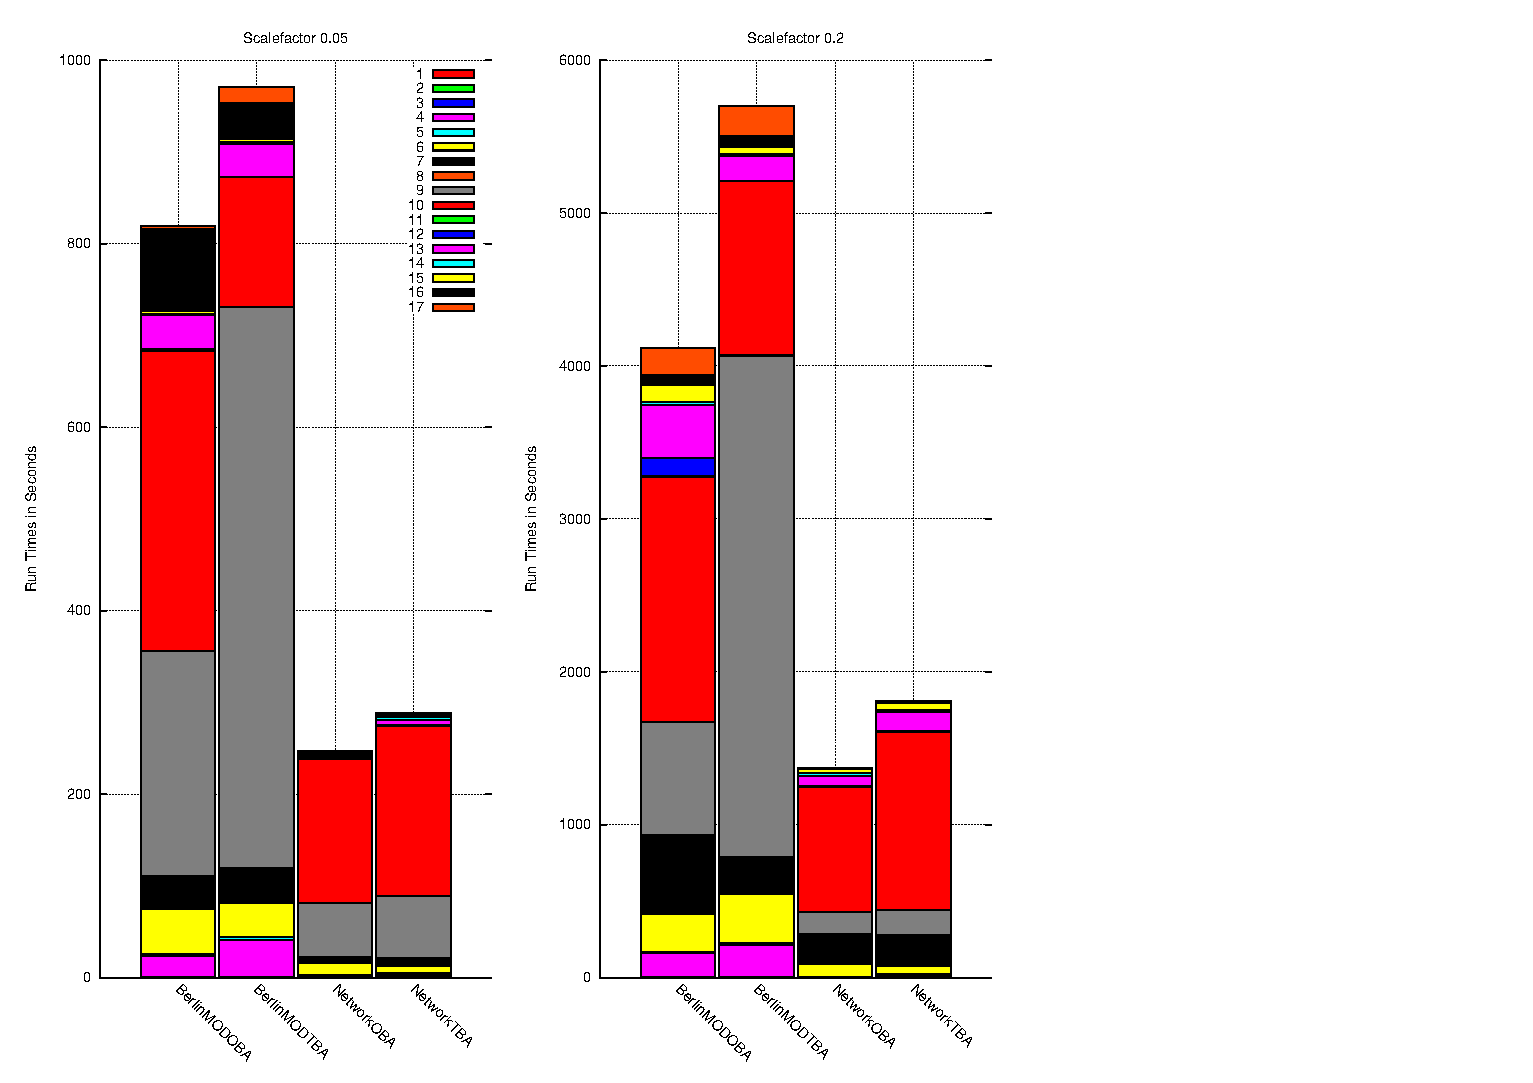
\includegraphics[width=17.0cm]{compruntimesall.eps}
	\caption{Compared Run Times for Each Query}
	\label{fig:compruntimesall}
\end{center}
\end{figure}

\section{New BerlinMOD Queries}
\label{sec:newqueries}
\section{Summary and Future Work}
\label{sec:summary}
Our experiments show that the network data model outperforms the \bmodb{} data model in the most cases. The good results of the network data model encouraged us to extend the \bmodb{} with a set of queries that enables us to compare the capabilities of different spatio-temporal network data models with respect to the specialised network challenges of this data models.

Actually we have a students practice group implementing a other network data model in \secondo{} DBMS. So that we will be enabled to compare the capabilities of the different network data models with the extended \bmodb{} in the near future.
\bibliography{BerlinMODAndNetworkDataModel}{}
\bibliographystyle{plain}
\end{document}
